
\chapter{The UQBT Framework}
\label{ch-uqbt-framework}

{\small
\begin{flushright}
Design: Cristina, Norman; Documentation: Cristina [c.98, May 00, Nov 01]
\end{flushright} 
}

The University of Queensland Binary Translator (UQBT) 
framework, is designed to support experimentation in static
binary translation.
UQBT strives to adapt easily to changes in both source and
target machines at low cost, including translations to
register-based and stack-based machines.
Support for multiple architectures is provided by means
of specification of properties of machines, as well as 
conventions used by operating systems.  
This chapter describes the overall architectural organization
of \uqbt\ (Section~\ref{sec-arch}) and its components from the point of view 
of instruction translation (Section~\ref{sec-framework}).  Note that
these two sections are necessarily overlapping; the former
section reflects more of the design and the latter section
reflects more of the implementation of the system.  
The chapter concludes with a small section on the state of the
UQBT framework at the end of 2001. 


\section{The Proposed 1997 Architecture of a Retargetable Binary Translator}
\label{sec-arch}

Like a compiler and a decompiler, a binary translator can logically
be divided into three phases: front end, analysis and transformation,
and back end.  For a given source machine M$_s$ and destination machine M$_d$,
the front end decodes machine M$_s$'s binary file and stores the 
information in a machine-independent intermediate form based on RTLs.
The analysis phase maps machine M$_s$'s locations onto machine M$_d$'s 
locations and transforms the RTLs so that they can be readily translated into 
native code for machine M$_d$.  The back end translates the intermediate 
form and writes a binary file for machine M$_d$.  It may also optimize 
instructions.

From a retargetability point of view, it is more helpful to think of 
a functional division into components instead of a sequential division 
into phases.  Such components may be used in more than one phase.
Some components will be machine-independent; others may be generated 
from machine descriptions.  In Figure~\ref{fig-architecture}, we identify 
components by putting them in boxes.

% original file created in Visio, printed to a file using Adobe's Default
% Postscript Printer driver (option EPS), and crop with ghostview (gsview 
% on the PC version 2.5) using File->PStoEPS option.
\centerfigbegin
\resizebox{!}{10cm}
{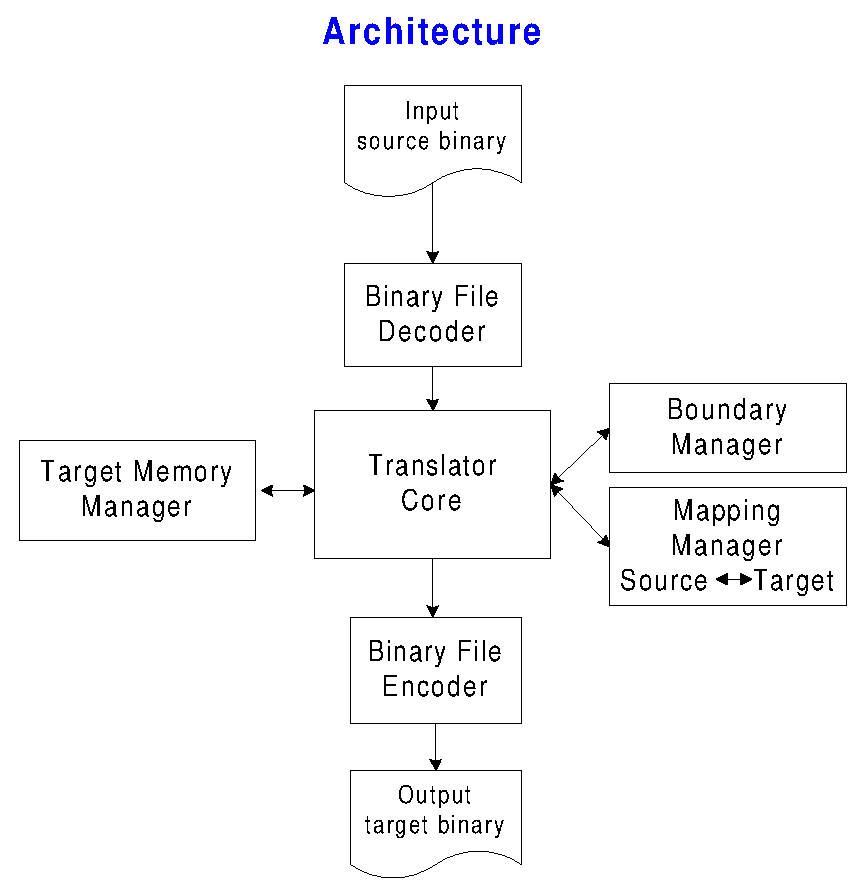
\includegraphics{figures/uqbt_architecture.eps}}
\centerfigend{fig-architecture}{Architecture for a Retargetable Binary
	Translator.  Components are Represented in Boxes.}

Implementation of components draws on techniques developed for
dcc, an 80286 decompiler~\cite{Cifu95}, for specifying
representations of machine instructions~\cite{Rams97},
and for the U.S. National Compiler Infrastructure project.


\subsection{Components}

M$_s$ \emph{binary file reader} exports an abstraction
representing the contents of the executable binary on the original
machine.  This module promotes retargetability by hiding
information about the source machine that one might otherwise be
tempted to exploit.  The capabilities exported include:
%\enumerateAlpha
\begin{enumerate}
\item The initial state of the M$_s$ processor that would apply when about
     to run this binary on a native M$_s$ processor, including at minimum
     the value of the program counter,
\item A list of potential entry points for procedures, possibly empty
     (N.B. the initial program counter is always available as an entry
     point), 
\item The ability to fetch the program's code and data, by the address
     those contents would occupy in a running M$_s$ executable, and 
\item The ability to identify calls to dynamically linked procedures, and
     to provide access to the code and data associated with those
     procedures.
\end{enumerate}
%\enumerateNumber
This module may therefore include much of the functionality of a dynamic
linker/loader.

One of the crucial decisions made by a translator is which locations
on machine M$_d$ hold what data from machine M$_s$.  We will encapsulate these
decisions in a \emph{mapping manager}, which will map locations in code
space, locations in data space, and locations referring to registers
or other processor state.  Most mappings will be determined
automatically at translation time, but some mappings may be specified
by hand for each pair of platforms, e.g., what registers of machine M$_d$
should be used to represent the contents of registers of machine M$_s$.

The mapping manager will rely on the M$_d$ \emph{memory manager} to allocate 
locations in the destination machine's storage space, e.g., to store 
translated code.

Because it is impossible to identify and translate all code, a running
image on machine M$_d$ will in general have a mix of translated and
untranslated code.  The \emph{boundary manager} will track the boundary
between translated and untranslated code and handle flow of control
across the boundary.  For example, a branch from translated to
untranslated code might go to an interpreter or to a dynamic
translator.  If the untranslated code is subsequently translated, the
boundary moves, and the boundary manager might backpatch the branch.

The \emph{core translator} will translate groups of machine instructions.
A group may be as small as a basic block or as large as an entire 
program, and different translation strategies (e.g., full static, 
partial static, dynamic) may use different group sizes.

The core translator coordinates the action of all the other
components and performs the main translation analyses.  It will 
translate a group of M$_s$ instructions as follows:
%\enumerateAlpha
\begin{enumerate}
\item Ask the memory manager for a location in M$_d$ to hold the translated
     code, and inform the mapping manager of the new mapping, 
\item Translate M$_s$ instructions to M$_d$ instructions
	  \begin{itemize}
      \item using information from the mapping manager to translate
         access to machine M$_s$'s data, 
      \item using information from the boundary manager to translate flow
	  \end{itemize}
	 of control outside the current group, and
\item Inform the boundary manager of the translation of the current group.
     The boundary manager may choose to backpatch branches into the
     current group.
\end{enumerate}
%\enumerateNumber
Depending on the granularity and timing of translation, these steps may
be repeated on other units until some termination condition is met.
If the granularity of translation is sufficiently large, the second step
may involve translating into an intermediate form and doing some global
analysis and optimization.

Finally, the M$_d$ \emph{binary file writer} will export an abstraction
representing the ability to create an executable binary on machine M$_d$.
It will export the abilities to:
%\enumerateAlpha
\begin{enumerate}
\item Specify the contents of the M$_d$ address space at the start of
     execution,
\item Establish the state of the M$_d$ processor at the start of execution,
\item Write an executable binary file in the M$_d$ native format, and
\item Possible support for dynamic linking, e.g. of translated or native
     libraries.
\end{enumerate}
%\enumerateNumber
In a dynamic translator, this component would simply write into a
running process image (and possible flush the I-cache).


\subsection{Core Translation based on RTLs}

The translation itself will be performed using register transfer lists
(RTLs).  An RTL is a collection of simultaneous effects.  Each effect
has the form `location := expression', and the expression is always
evaluated without side effects, so all state change is explicit.  
RTL expressions are represented as trees, the leaves of which refer to
constants or to the values contained in locations.  Note that although
the tree leaves refer to locations, the values themselves are not
necessarily calculated, only the location is referenced.
The internal nodes of the trees are `RTL operators'.  
For illustrative purposes, the following is an ASCII representation of an 
RTL representing the effect of the SPARC \texttt{andcc} instruction:
\begin{smallverbatim}
 $r[rd] <--      and (*$r[rs1], if i = 0 then *$r[rs2] else simm13! fi);
 icc.N  <-- bit (and (*$r[rs1], if i = 0 then *$r[rs2] else simm13! fi) < 0);
 icc.Z  <-- bit (and (*$r[rs1], if i = 0 then *$r[rs2] else simm13! fi) = 0);
 icc.V  <-- 0;
 icc.C  <-- 0
\end{smallverbatim}
This RTL does a bitwise AND of the contents of register rs1, either
with the contents of register rs2 or with a signed immediate value (simm13).
This result is stored in register rd, and it is also used to set two
of the four condition codes.  The other two condition codes are set to 
zero by the instruction.

RTLs are obviously complex and detailed.  Machine descriptions
themselves will be written at a higher level of abstraction and
compiled into RTLs.  Run-time representations of RTLs will be
`collapsed' either by analyzing these higher-level representations or
by using the `superoperator' technique~\cite{Proe95}.  
For example, we might define a superoperator LOGICAL such that LOGICAL(X)
stood for
\begin{smallverbatim}
 $r[rd] <--      X;
 icc.N  <-- bit ((X) < 0);
 icc.Z  <-- bit ((X) = 0);
 icc.V  <-- 0;
 icc.C  <-- 0
\end{smallverbatim}
Such a superoperator could be derived from the SPARC description. 

An `RTL language' is defined by a collection of locations and
operators.  For binary translation, a suitable RTL language can be
defined by taking the union of locations on machines M$_s$ and M$_d$ and the
union of the operators used in the descriptions of machine M$_s$ and M$_d$.
The `machine X invariant' defines a sub-language of RTLs called the
X-RTLs; an RTL is an X-RTL if and only if it can be represented as a
single instruction on machine X.

% original figure in Visio, exported as eps (without including TIFF
% preview or background rectangle).
\centerfigbegin
\resizebox{!}{12cm}
{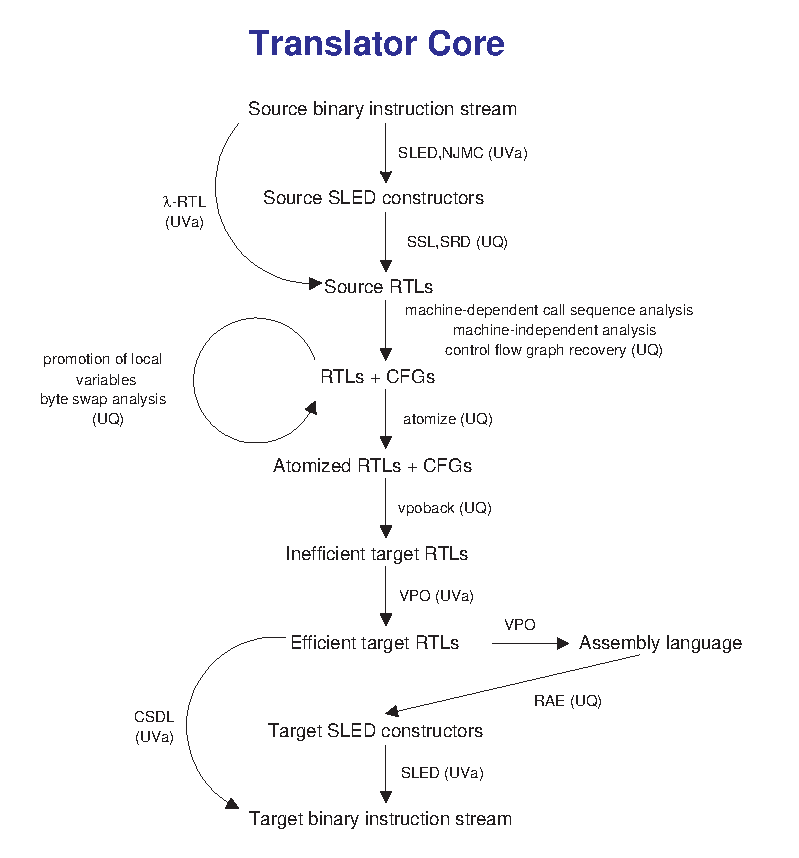
\includegraphics{figures/uqbt_dataflow.eps}}
\centerfigend{fig-dataflow}{Flow of Data through the System}

As shown in Figure~\ref{fig-dataflow}, the main steps in the translation are:
\begin{enumerate}
\item Decode the binary stream into M$_s$-RTLs.  This step will be
     automated by specifying syntax and semantics of M$_s$ instructions.

\item Build a control flow graph (CFG) for each procedure.  Analysis
     will be needed to find code associated with a procedure.

\item With the help of the mapping manager, map the machine M$_s$ locations
     in the RTLs to machine M$_d$ locations or to temporaries.

\item `Atomize' the RTLs to expose all RTL operators at top level, and
     find suitable replacements for machine M$_s$ operators that are not
     available on machine M$_d$.  For example, big-endian memory access
     might be replaced with explicit byte swapping.

\item Reassemble the RTLs to satisfy the machine M$_d$ invariant, making
	them M$_d$-RTLs (i.e. M$_d$-RTLs have a 1:1 mapping with M$_d$ 
	assembly instructions).

\item Optimize the M$_d$-RTLs using VPO~\cite{Beni88} or any other RTL 
	optimizer.

\item Encode the M$_d$-RTLs into binary code for machine M$_d$.  Also automated.
\end{enumerate}

The most challenging steps are steps (4) and (5).  In the initial
stages, these will be implemented by hand; we hope to develop automated
techniques afterwards.  The other steps can be automated based on
machine descriptions or a mapping specification.

Future analyses, intended to improve translated code, might be
implemented after steps (2), (3), or (4).  Such analyses might make it
possible to avoid byte swapping, to use machine M$_d$ calling conventions,
to put machine M$_s$ stack variables in machine M$_d$ registers, etc.
Analyses may vary depending on the granularity of translation.


\section{The 1999 UQBT Framework}
\label{sec-framework}

In order to support resourceability and retargetability, 
machine descriptions of machine properties are needed, 
as well as descriptions of conventions and formats used by 
the operating system.  We have identified 6 different specification 
languages and/or APIs to support the UQBT framework, 4 of these are 
currently in use in our framework. 

The framework described in this section dates from 1998, 
Section~\ref{sec-2001framework} describes the 2001 framework. 
References in this section are to papers and chapters within 
this book that explain in more detail a particular concept. 


\subsubsection*{Machine specifications and APIs} 
Properties of a machine are represented in terms of the machine 
instructions (i.e. the mnemonics), the semantics of such instructions, 
the identification of the instructions that transfer flow of control, 
and, if needed, delayed transfers of control information.  
These 4 types of information are represented by the following 
languages: 

  \begin{itemize}
  \item SLED (Specification Language for Encoding and Decoding), 
	which supports descriptions of the syntax of machine 
	instructions~\cite{Rams97}.  [Chapter~\ref{ch-decoding}];

  \item SSL (Semantic Specification Language), which supports 
	descriptions of the semantics of machine 
	instructions~\cite{Cifu98c}.  [Chapter~\ref{ch-ssl}]; 

  \item CTL (Control Transfer Language), which supports the 
	identification of instructions that perform control 
	transfers of control (conditional jumps, jumps, calls or 
	returns). This language was implemented as a loose API in the
	end, as we decided not to specify other transfer of control 
	information in the end.  

  \item DCTL (Delayed Control Transfer Language), which supports 
	the description of simple transformations needed in 
	order to remove dependencies on delayed instructions (in 
	machines that support such concept).  

    Support for DCTL is not in place at present.  Initially, we used 
    a program-transformation and partial-evaluation technique to derive 
    the transformations on instructions that support delayed transfers of 
    control~\cite{Cifu98i}.  [Chapter~\ref{ch-delay}].
    The code is voluminous and we believe that code to support such 
    transformations could be automated from a short specification 
    of the required transformations.  This step would clearly increase 
    the resourceability of the framework.  However, we note that not 
    too many machines currently support the delayed-slot transfer of 
    control, only SPARC, PA-RISC and MIPS do at present time.

  \end{itemize}


\subsubsection*{OS specifications/APIs} 
Conventions and formats used by a multiplatform operating system come 
in the form of calling conventions, including where parameters are passed 
(i.e. stack or registers), and the format of the binary-file that the 
OS supports.  
These 2 pieces of information are represented by the following 
languages/APIs: 

  \begin{itemize}
  \item PAL (Procedural Abstraction Language), which supports 
	the description of calling conventions, parameter passing conventions, 
	and local variables conventions~\cite{Cifu99g}. [Chapter~\ref{ch-call}];  
	and 

  \item BFF (Binary File Format), which supports the description 
	of the internal format of a binary-file, such as the 
	Elf format on Solaris and Linux systems~\cite{Cifu97f}. 
	[Chapter~\ref{ch-bff}].  
  \end{itemize} 

We currently support the PAL language and have worked on 
an initial prototype of the BFF language, which is incomplete 
at present time but proves the feasibility of specifying 
binary-file formats and automatically generating code to 
support the decoding of such files.  In our experience, it 
was easier to have a set API for dealing with differences in 
binary-file formats than to specify the existing ones.   

\psfigbegin{figures/uqbtImplementation.eps}{10cm}
\psfigend{fig-uqbt}{Framework for a Resourceable Binary Translator.}

Figure~\ref{fig-uqbt} illustrates the components of the 
translation process in the form of boxes.  Specifications for different
machines are illustrated with the document shape.
Greyed-out shapes mean that they are not currently supported 
by UQBT and therefore an implementation for a particular format 
or analysis has been done instead.  Arrows represent conceptual 
flow of control in the translation process.  


\subsection{The Decoding Phase}
The binary-file decoder, instruction decoder 
and semantic mapper translate raw machine instructions into  
M$_s$-RTLs for a given source machine M$_s$.  
As previously mentioned, we consider M$_s$-RTLs machine dependent, as
they represent how the source machine performs a given instruction, 
including delayed-slot semantics for example.  

In static translators, the amount of decoding from this phase 
is limited by indirect transfers of control (i.e. statically,  
it is not always possible to determine the target of an 
indexed jump or an indirect call).  
UQBT includes a slicing-based technique to determine the target
address(es) of indirect transfers of control~\cite{Cifu99c}. 
This technique allows us to decode a larger percentage of the
code than otherwise possible, and is reusable across different 
platforms.  


\subsection{The Analysis Phase} 
The translation of M$_S$-RTLs up to \hrtl\ is 
the most challenging stage of the translator.  As seen in 
Figure~\ref{fig-uqbt}, this translation requires information 
about control transfer instructions, delayed control transfers 
(if any), parameter and calling conventions, and locals and 
stack frame conventions.  
CTL specifications allow us to translate low-level register 
transfers into higher level instructions such as calls and 
returns.  
For example, a CTL specification for SPARC states that a 
jump and link instruction with destination register \texttt{\%o7} 
is a call instruction.  This semantics is not necessarily 
obvious from the SSL description of a jump and link instruction. 
Further, the same instruction using destination register 
\texttt{\%g0} is equivalent to an unconditional jump; this 
too is specified in CTL.  

DCTL specifications will allow us to remove delayed-slot 
instructions in a more machine-independent way.  
At present, as previously mentioned, we implement a program
transformation and partial evaluation technique. 

PAL specifications allow us to recover some of the high-level nature 
of the code, by recovering actual parameters and return 
values for functions, and removing the M$_S$-RTL-specific 
instructions that form part of procedure prologues and 
epilogues, as these are represented in different ways in 
different machines.  The analysis is based on live and 
used parameter and return locations; such locations being
specified in a PAL specification, as well as abstraction to 
an abstract frame pointer (\texttt{\%afp}).  
For example, a PAL specification for the Pentium would specify
that parameters can be passed on the stack and that return 
values go into certain registers (\texttt{\%eax} and top of 
the floating point stack). 
A more detailed description of the analysis is available 
in~\cite{Cifu99g} and Chapter~\ref{ch-call}. 
 
\centerfigbegin
\begin{fnverbatim}
r[tmp] = %sp
r[tmp2] := -120
%pwp = %cwp
%cwp = %cwp + 64
%cwp = (%cwp-1) % NWINDOWS
%sp = r[tmp] + r[tmp2]
r[9] = 69 << 10            v1 = 70656
r[8] = r[9] | 720          v0 = v1 | 720
r[15] = %pc
%pc = %npc
%npc = 0x21780             Call printf (v0, v1)
r[9] = r[30] + -20         v1 = %afp + 100
r[10] = 69 << 10           v2 = 70656
r[8] = r[10] | 736         v0 = v2 | 736
r[15] = %pc
%pc = %npc
%npc = 0x2178c             Call scanf (v0, v1, v2)
r[8] := m[r[30] - 20]      v0 = m[%afp + 100]
r[15] = %pc
%pc = %npc
%npc = 0x10a9c             v0 = Call fib (v0)
m[r[30] - 24] = r[8]       m[%afp + 96] = v0
\end{fnverbatim}
\centerfigend{fig-palEg}{Example of the result of the use of PAL
        specifications to translate SPARC-RTL code (left-hand side)
        to \hrtl\ (right-hand side) in a fibonacci program.}

Figure~\ref{fig-palEg} illustrates 
a snippet of SPARC-RTLs for the \texttt{main} of a fibonacci 
program, and the resultant \hrtl\ code.  As can be seen, 
the RTLs for the procedure prologue were removed (and relevant information
used in the translation), the actual parameters to library functions 
\texttt{printf} and \texttt{scanf} are listed, actual parameters 
were moved to variable locations, local variables are in terms of 
an abstract frame pointer called \texttt{\%afp}, and the return 
value for the call to \texttt{fib} has been determined.   
The example also shows that the call to \texttt{fib} has the
right number of parameters (i.e. one), and that the calls to
the variable argument routines \texttt{printf} and \texttt{scanf} 
each take one extra parameter than expected.  These parameters were passed 
as they were live and were valid parameter locations at the 
call site.  However, when the code is executed, these parameters
will not be used as the library routines would not be expecting
these parameters for processing (i.e. the format string 
in both these routines specifies the number of parameters
required to be processed), therefore producing the right
result at runtime.  

Lifting the level of representation of the code to \hrtl\ 
allows for experimentation with different types  
of binary translation-specific optimizations, such as removing 
some of the byte swaps at loads and stores when machines have  
different endianness, or promoting local variables to registers. 
This is future work. 


\subsection{The Encoding Phase} 
\label{sec-encoding}

\centerfigbegin
\begin{fnverbatim}
void main() {
int v0;
int v1;
int v2;
char _locals[120];

        v1=70656;
        v0=(v1)|(720);
        printf(v0,v1);
        v1=(_locals)+(100);
        v2=70656;
        v0=(v2)|(736);
        scanf(v0,v1,v2);
        v0=*((int*)((_locals)+(100)));
        v0=fib(v0);
        *((int*)((_locals)+(96)))=v0;
\end{fnverbatim}
\centerfigend{fig-cEg}{Example generated low-level C code for the partial
        fibonacci example of Figure~\ref{fig-palEg}.}

The last step in this phase is the translation down to the 
target machine's intermediate representation; M$_T$-RTL in 
the case of register-based machines or \bcode\ in the case 
of stack-based machines.  
The translated code will always require an optimizer to improve 
its quality, therefore, the encoder phase would be equivalent 
to that of an optimizing compiler.  Because we interface 
to existing C optimizing compilers, we generate very low-level 
C code from this step.  Figure~\ref{fig-cEg} shows the 
generated low-level C code for the example in Figure~\ref{fig-palEg}. 
As can be seen, data addresses are not modified, therefore  
a call to \texttt{printf} or \texttt{scanf} takes the same 
memory address as that in the source binary.  

We have successfully interfaced to VPO~\cite{Beni88}, whose register 
transfer list interface is similar to our RTLs, and hence it is simple  
to translate to.  The new VPO interface is part of the Zephyr 
project~\cite{Vpo98}.  
Generating (low level) C allows us to experiment with different 
optimizers, and also is the interface to the stack based backends. 
For generation of code to the Java Virtual Machine (JVM), we 
have written a backend and a bytecode description that 
integrates with gcc. 

\centerfigbegin
\begin{fnverbatim}
                   ... (setup code)
v2=134517960;      ldc 124517960   ; put string in local 10
printf(v2);        istore 10
r24=(_afp)+(4);    aload_0         ; call _printf
v2=r24;            iload 10
v1=134517975;      invokevirtual Fibo/_printf (I) I
scanf(v1,v2);      istore 10
                   ldc 16          ; put afp+4 in local 12
                   lstore 9
                   iload 14
                   iload 9
                   iadd
                   istore 12
                   ldc 134517975   ; put string in local 10
                   istore 10
                   iload 12        ; put afp+4 in local 11
                   istore 11
                   aload_0         ; call _scanf
                   iload 10
                   iload 11
                   invokevirtual Fibo/_scanf(II)I
                   istore 10
\end{fnverbatim}
\centerfigend{fig-bcodeEg}{Example of generated bytecode after gcc
        optimizations (right-hand side) for low-level C code
        generated from Pentium fibonacci binary (left-hand side).}

The generation of bytecode via gcc provides us with all the
classical optimizations that are too computationally expensive to be
performed by a just-in-time compiler.  
We wrote a bytecode specification file for gcc which treats registers 
as locals and describes peephole optimizations.  
For each \hrtl\ instruction, $n$ bytecode instructions are 
generated, where $n$ is normally less than 5.  The generated
bytecode is similar to that generated by a Java compiler, 
given the high level of abstraction of the \hrtl\ code.  
Current work under development improves on the generated bytecode 
by using an intermediate language called \bcode, which allows 
for stack-based optimizations to be performed, therefore minimizing the 
amount of loads and stores from memory and using the stack 
for temporary values more. 
Figure~\ref{fig-bcodeEg} shows sample bytecode generated from our 
gcc bytecode backend.  Library calls are to wrapping routines 
which invoke the native Java library subsystems.  For variable
argument routines, we have $n$ different wrappers, where $n$ is
the number of parameters and typically $n$ is less than 10. 

For each translation, the generated code and data are 
placed into a variety of C and assembly files which can be 
compiled with gcc and gas on the target machine.  
For each function, a low-level C file is generated. 
For each data section, an assembly file is generated with the  
relevant bytes. 
A makefile is provided to pack the file into an appropriate 
binary for the target machine.

Static translators require the use of an interpreter/emulator to handle 
untranslated code that is discovered at run time.  
The interpreter uses the M$_S$-to-M$_T$ mapping to determine when 
it can return to translated code, and therefore this mapping is stored 
in the target binary.
Because the interpreter will use the original source text section, 
this section is also copied to the target binary.
The interpreter itself is designed to be linked dynamically.
We are currently building a resourceable interpreter/emulator which uses 
the same SLED and SSL specifications provided by the UQBT framework.
The interpreter simulates M$_s$-RTLs and uses PAL specifications 
to determine how to pass parameters to library routines.  
This work is not completed at present time and is under development.

Because of potential aliasing problems, not all of which can be solved by
static analysis, the data sections (generally .rodata and .data in 
Elf binary files) are copied ``as is'' to the target binary. 
They are made to retain the same Virtual Memory Address in the 
target binary as in the source binary. A link map file generated by 
the translator is used to achieve this. The target program calculates 
addresses exactly as the original source program did, and so the data 
is referenced correctly (although it may need to be referenced 
using different endianness). 
Because of differences in size of pages in various architectures 
(e.g. 4Kb on Pentium, verses typically 8Kb on SPARC), this mapping 
cannot always be achieved entirely by manipulation of addresses in the 
target binary file. A very small piece of code sometimes has to perform block 
moves (before the normal startup code) to achieve the correct addresses.

Translators to bytecode require extra environment support
to compliment the strengths of the JVM.  The lack of a generic memory
model on the JVM forces us to emulate the data and stack of a translated
program.  Library functions from the source architecture must also be
supplied to the translated program.  This is facilitated by a superclass
from which each translated program is inherited.  The superclass provides
simulated memory access in preloaded byte arrays and wrapper routines to 
library functions which invoke the native Java subsystems.


\section{The 2001 UQBT Framework}
\label{sec-2001framework}

\psfigbegin{figures/uqbtOverall2001.eps}{10cm}
\psfigend{fig-uqbt2001}{The 2001 UQBT Framework}

The final UQBT 2001 framework provides for several backends that 
were written for experimentation with different ways of generating 
machine code, by integrating at different levels of abstraction. 
Figure~\ref{fig-uqbt2001} shows this framework, we briefly describe
its components next.  In the below description, we divide the framework 
into two sections, the front end and the back end.  The former transforms
binary code to the \hrtl\ representation, the latter transforms down 
from \hrtl\ into another binary representation.

\begin{description}
\item Front end: 
We have one resourceable front end which takes 3 machine and OS 
descriptions and 2 APIs, along with any extra machine-dependent 
code to abstract M$_s$-RTLs into \hrtl\ code.  The parts of the 
front end are: 

\begin{itemize}
\item Binary-file decoder: supports the decoding of the source 
	binary file into an internal UQBT representation that supports 
	the binary-file format API.  The API assumes we can obtain the 
	code (text) and data sections of the file, that there is at 
	least one entry point, and that there may be a symbol table.  

\item Instruction decoder: supports the disassembly of the instruction 
	stream (the text/code section(s)) via the SLED specification for
	the instruction set for the source machine being used.   

\item Semantic mapper: supports the conversion of assembly instructions 
	into RTL instructions, by implementing support for the SSL language, 
	which describes the semantics of assembly instructions. 

\item M$_s$-RTL to \hrtl\ translator: this is the key module in the
	framework that allows us to obtain machine independence in the 
	representation of the code of the program.  This module transforms 
	RTL instructions into \hrtl\ instructions, by supporting an 
	informal control transfer API, performing analyses on procedural  
	information (such as parameters, locals and return locations), 
	and adding any extra hand-written code to support peculiarities 
	of the source instruction set; such as delayed branches on SPARC 
	or floating point stack-based instructions on x86.    
\end{itemize}

The net result of the front end phase is to transform the source 
binary's code into a \hrtl\ representation which is machine independent. 
Transformations on this representation are feasible in order to, 
for example, reduce the number of byte swaps needed when translating 
to different endianness machines.  Transformations of this kind are 
considered binary translation-specific optimizations, as a traditional 
compiler optimizer would not have to deal with them at all.  

\item Back end: 
We have experimented with four different types of back ends.  These 
back ends have commonalities which could be extracted into a common 
back end that supports generation of code at different levels of 
abstraction (such as RTL, assembly or object code).  The back ends are:  

\begin{itemize}
\item C back end: the C backend was the original back end we wrote 
	for the UQBT framework that supported several target platforms 
	(we had earlier experimented with an RTL optimizer).  
	In essence, the C compiler was used as a macro assembler.  
	We translated \hrtl\ code into low-level C code; 
	i.e. code that makes use of goto's and performs a lot of casting 
	of types of expressions.  The generated low-level C code would then 
	be compiled and optimized by the C compiler (we normally compiled 
	using GNU's gcc as well as Sun's cc compilers) and then linked 
	against the original data sections of the source program.  The data 
	sections were always forced to be located at the same memory address 
	space as in the original source program.  

\item JVML back end: the Java bytecode (Java virtual machine language (JVML)) 
	back end was written as an experiment in translating machine code to 
	Java bytecodes.  We translated \hrtl\ code into Java bytecode assembly 
	code, which would be assembled by the Jasmin assembler in order to 
	generate a Java binary (.class file).  Some runtime support was needed 
	as the JVM model is different to that of traditional machines; there 
	was support for dealing with memory, allocating and deallocating memory, 
	as well as support for 32-bit integrals (all integers in the JVM model 
	use 31 bits and are meant to be signed).

\item RTL back end: the RTL back end was an experiment at having more 
	control over the optimizations that were applied to the generated 
	code, as by generating RTL instructions for the target machine, 
	we could then tell an RTL-optimizer to only use certain optimizations 
	and to not move around code in certain sections.   We used the 
	VPO~\cite{Beni88} system for this purpose.  VPO is a retargetable 
	optimizer that now provides an RTL interface to it.  VPO makes use 
	of specifications to describe the syntax of the target instructions, 
	has a series of optimizations that are machine independent, and 
	requires the user to write machine dependent optimizations to support 
	any new machine.  

\item Object code back end: the object code back end was written as an 
	experiment to interface with an optimizer at the object code level, 
	i.e. without having to generate any particular intermediate 
	representation.  The generated code would not do register allocation 
	of any sort, instead, it would place all locations (variables and 
	registers) onto the local stack of a procedure, and would rely on 
	the optimizer to perform register allocation.  This was an internal 
	Sun experiment that made use of a proprietary optimizer, as such, 
	the code is released in the event that it is useful to others, but
	the code for the optimizer is not made available (you can potentially
	interface with any optimizer you see fit).   
\end{itemize}


\end{description}


